\chapter{Multilevel K-Way Graph Partitioning}\label{chap:multilevel-kway}
This chapter presents the Multilevel K-way Graph Partitioning algorithm which is one of the most widespread GP algorithms. Each section will explain in detail the phases of the multilevel approach with special focus on the techniques used in the partitioner used in this thesis.  

\section{Preliminaries}
The overall structure of a multilevel k-way graph partitioning algorithm is fairly straightforward. The process begins by coarsening the input graph until it is reduced to a size of only a few thousand vertices. At this coarsest level, an initial k-way partitioning is computed using
graph growing algorithm (see Section~\ref{graph_growing})~\cite{KarypisGeorge1998AFaH}. The graph is then uncoarsened back to its original size in successive steps. At each level of uncoarsening, the partitioning is refined to improve quality by exploiting the increased degrees of freedom available at the finer level. Karypis and Kumar demonstrate in~\cite{karypis_multilevelk-way_1998} that this multilevel approach yields high quality partitions, often comparable to, or better than, those produced by recursive bisection~\cite{KarypisGeorge1998AFaH}.

In Figure~\ref{fig:multilevel-overview}, this process is illustrated showing how an initial graph $G_0$ is coarsened until it reaches $G_4$ which is smaller in size. At this level an initial partition is performed on the coarsest graph. After that the graph is step by step projected back to its original size, refining the partition at each level in order to minimize the chosen objective function~\cite{KarypisGeorge1999PMkP}.

The multilevel partitioning problem uses the same definitions as in Section~\ref{sec:gpp}. Additionally, we represent a k-way partition through a vector $P$. The vector has a length of $n$, where $n$ is the number of vertices in the graph. Each element of \textit{P} is an integer between 1 and $k$, indicating the partition the vertex belongs to. Specifically, a vertex $v \in V$ assigned to partition \textit{a} will have $P[v] = a$. The next sections will now explain how each phase works and how the partitions are formed. 

\begin{figure}[h]
	\centering
	\scalebox{0.65}{\begin{tikzpicture}[
	graph label/.style={font=\large},
	phase arrow/.style={-{Stealth[length=8pt]}, thick, black},
	phase label/.style={font=\Large\bfseries, text=red},
	pline/.style={green!70!black, thick},
	]
	
	% LEFT SIDE - Coarsening phase
	% G0
	\begin{scope}[shift={(-5, 8)}]
		\draw[thick, fill=white] plot[smooth cycle, tension=0.4] coordinates {
			(1.8, 0)    (1.5, 0.8)   (1.2, 1.1)   (0.0, 1.2)
			(-0.9, 1.0) (-1.3, 0.5)  (-1.8, -0.1) (-1.3, -0.9)
			(-0.7, -1.1) (0.1, -1.2) (1.0, -0.9)  (1.7, -0.4)
		};
		\node[graph label] at (0,0) {$G_0$};
	\end{scope}
	
	% G1
	\begin{scope}[shift={(-4, 5)}]
		\draw[thick, fill=white] plot[smooth cycle, tension=0.4] coordinates {
			(1.5, 0)    (1.25, 0.67)  (1.0, 0.92)   (0.0, 1.0)
			(-0.75, 0.83) (-1.08, 0.42) (-1.5, -0.08) (-1.08, -0.75)
			(-0.58, -0.92) (0.08, -1.0) (0.83, -0.75)  (1.42, -0.33)
		};
		\node[graph label] at (0,0) {$G_1$};
	\end{scope}
	
	% G2
	\begin{scope}[shift={(-3, 2)}]
		\draw[thick, fill=white] plot[smooth cycle, tension=0.4] coordinates {
			(1.3, 0)     (1.08, 0.57)  (0.87, 0.78)   (0.0, 0.85)
			(-0.65, 0.71) (-0.94, 0.35) (-1.3, -0.07) (-0.94, -0.64)
			(-0.51, -0.78) (0.07, -0.85) (0.72, -0.64)  (1.23, -0.28)
		};
		\node[graph label] at (0,0) {$G_2$};
	\end{scope}
	
	% G3
	\begin{scope}[shift={(-2, -0.8)}]
		\draw[thick, fill=white] plot[smooth cycle, tension=0.4] coordinates {
			(1.0, 0)     (0.83, 0.47)  (0.67, 0.64)   (0.0, 0.7)
			(-0.5, 0.58) (-0.72, 0.29) (-1.0, -0.06) (-0.72, -0.52)
			(-0.39, -0.64) (0.06, -0.7) (0.56, -0.52)  (0.94, -0.23)
		};
		\node[graph label] at (0,0) {$G_3$};
	\end{scope}
	
	% G4 with initial partition
	\begin{scope}[shift={(0.5, -3)}]
		\draw[thick, fill=white] plot[smooth cycle, tension=0.4] coordinates {
			(0.75, 0)     (0.63, 0.37)  (0.5, 0.5)    (0.0, 0.55)
			(-0.38, 0.46) (-0.54, 0.23) (-0.75, -0.05) (-0.54, -0.41)
			(-0.29, -0.5) (0.04, -0.55) (0.42, -0.41)  (0.71, -0.18)
		};
		\node[graph label] at (-1.2, -0.0) {$G_4$};
		\draw[green, thick] (-0.42, 0.41) to[out=-90, in=60]
		coordinate[pos=0.35](p1) (-0.54, -0.41);
		\draw[green, thick] (p1) to[out=-27, in=98]
		coordinate[pos=0.35](p2) coordinate[pos=0.65](p3) (0.42, -0.41);
		\draw[green, thick] (p2) to[out=45, in=-90] (0.5, 0.5);
		\draw[green, thick] (p3) to[out=-30, in=140] (0.71, -0.18);
	\end{scope}
	
	% RIGHT SIDE - Uncoarsening phase
	% G3 right
	\begin{scope}[shift={(3, -0.8)}]
		\draw[thick, fill=white] plot[smooth cycle, tension=0.4] coordinates {
			(1.0, 0)     (0.83, 0.47)  (0.67, 0.64)   (0.0, 0.7)
			(-0.5, 0.58) (-0.72, 0.29) (-1.0, -0.06) (-0.72, -0.52)
			(-0.39, -0.64) (0.06, -0.7) (0.56, -0.52)  (0.94, -0.23)
		};
		\node[graph label] at (0,-0.35) {$\small G_3$};
		
		\draw[green, thick] (-0.56, 0.52) to[out=-90, in=60]
		coordinate[pos=0.35](p1) (-0.72, -0.52);
		\draw[green, thick] (p1) to[out=-27, in=98]
		coordinate[pos=0.35](p2) coordinate[pos=0.65](p3) (0.56, -0.52);
		\draw[green, thick] (p2) to[out=45, in=-90] (0.67, 0.64);
		\draw[green, thick] (p3) to[out=-30, in=140] (0.94, -0.23);
	\end{scope}
	
	% G2 right
	\begin{scope}[shift={(4.5, 2)}]
		\draw[thick, fill=white] plot[smooth cycle, tension=0.4] coordinates {
			(1.3, 0)     (1.08, 0.57)  (0.87, 0.78)   (0.0, 0.85)
			(-0.65, 0.71) (-0.94, 0.35) (-1.3, -0.07) (-0.94, -0.64)
			(-0.51, -0.78) (0.07, -0.85) (0.72, -0.64)  (1.23, -0.28)
		};
		\node[graph label] at (0,-0.35) {$G_2$};
		% Wavy horizontals
		\draw[green, thick] (-0.72, 0.64) to[out=-90, in=60]
		coordinate[pos=0.35](p1) (-0.94, -0.64);
		\draw[green, thick] (p1) to[out=-27, in=98]
		coordinate[pos=0.35](p2) coordinate[pos=0.65](p3) (0.72, -0.64);
		\draw[green, thick] (p2) to[out=45, in=-90] (0.87, 0.78);
		\draw[green, thick] (p3) to[out=-30, in=140] (1.23, -0.28);
	\end{scope}
	
	% G1 right
	\begin{scope}[shift={(5.5, 5)}]
		\draw[thick, fill=white] plot[smooth cycle, tension=0.4] coordinates {
			(1.5, 0)    (1.25, 0.67)  (1.0, 0.92)   (0.0, 1.0)
			(-0.75, 0.83) (-1.08, 0.42) (-1.5, -0.08) (-1.08, -0.75)
			(-0.58, -0.92) (0.08, -1.0) (0.83, -0.75)  (1.42, -0.33)
		};
		\node[graph label] at (0,-0.5) {$G_1$};
		% Wavy verticals
		\draw[green, thick] (-0.83, 0.75) to[out=-90, in=60]
		coordinate[pos=0.35](p1) (-1.08, -0.75);
		\draw[green, thick] (p1) to[out=-27, in=98]
		coordinate[pos=0.35](p2) coordinate[pos=0.65](p3) (0.83, -0.75);
		\draw[green, thick] (p2) to[out=45, in=-90] (1.0, 0.92);
		\draw[green, thick] (p3) to[out=-30, in=140] (1.42, -0.33);
	\end{scope}
	
	% G0 right
	\begin{scope}[shift={(6.5, 8)}]
		\draw[thick, fill=white] plot[smooth cycle, tension=0.4] coordinates {
			(1.8, 0)    (1.5, 0.8)   (1.2, 1.1)   (0.0, 1.2)
			(-0.9, 1.0) (-1.3, 0.5)  (-1.8, -0.1) (-1.3, -0.9)
			(-0.7, -1.1) (0.1, -1.2) (1.0, -0.9)  (1.7, -0.4)
		};
		\node[graph label] at (0,-0.6) {$G_0$};
		
		% Partition curves using explicit boundary coordinates
		% 150° ≈ (-1.3, 0.5), 220° ≈ (-1.3, -0.9), 310° ≈ (1.0, -0.9), 60° ≈ (1.2, 1.1)
		
		\draw[green, thick] (-1.0, 0.9) to[out=-90, in=60]
		coordinate[pos=0.35](p1) (-1.3, -0.9);
		
		\draw[green, thick] (p1) to[out=-27, in=98]
		coordinate[pos=0.35](p2) coordinate[pos=0.65](p3)
		(1.0, -0.9);
		
		\draw[green, thick] (p2) to[out=45, in=-90]
		(1.2, 1.1);
		
		\draw[green, thick] (p3) to[out=-30, in=140]
		(1.7, -0.4);
	\end{scope}
	
	% Large curved phase arrows
	\draw[-{Stealth[length=10pt]}, very thick, black]
	(-6.4, 5.9) .. controls (-7.7, -1) and (-6, -1) .. (-2.5, -2.8);
	
	\draw[-{Stealth[length=10pt]}, very thick, black]
	(2.5, -2.8) .. controls (7.1, -1) and (8.8, -1) .. (7.5, 5.9);
	
	% Phase labels
	\node[phase label, rotate=90] at (-7.9, 4) {Coarsening phase};
	\node[phase label] at (0.5, -4.8) {Initial partitioning phase};
	\node[phase label, rotate=-90] at (9.5, 4) {Uncoarsening phase};
	\node[font=\Large\bfseries, text=black!80!black] at (0.5, 10.2) {Multilevel \textit{k}-Way Partitioning};
	
\end{tikzpicture}}
	\caption{The phases of the multilevel k-way partitioning algorithm. During the coarsening phase, the vertices are contracted together and the graph size is successively decreased; during the initial partitioning phase, a k-way partition is performed on the smallest graph; and during the uncoarsening phase, the partitions are successively refined and projected back to a larger graph.}
	\label{fig:multilevel-overview}
\end{figure}

\section{Coarsening Phase}
During the coarsening phase, a sequence of increasingly smaller graphs is constructed maintaining a similar structure to the original graph with fewer degrees of freedom. The most common approach is to aggregate groups of vertices into a single coarse vertex through matching~\cite{buluc_recent_2016, KarypisGeorge1998AFaH}. The coarse vertex has a weight equal to the sum of the weights of all the vertices it contains. Additionally, the coarse vertex receives all the edges of the vertices it contains. Vertices that are not matched are simply copied over to the smaller graph. This process is repeated until we reach a graph $G_m$ with a small enough number of vertices~\cite{karypis_analysis_1995}.

For a given graph $G_i = (V_i, E_i)$, a subset of vertices $V^v_i \subseteq V_i$ is merged into a coarse vertex $v \in V_{i+1}$ for the next coarser graph $G_{i+1}$. The coarse vertex $v$ has weight $w(v) = \sum_{u \in V^v_i}w(u)$. This ensures that the total vertex weight is preserved across coarsening levels. To preserve connectivity, the new vertex $v$ receives the union of the edges of the vertices in $V^v_i$. For any neighbor vertex $u$, the edge weight is $w(\{v,u\}) = \sum_{z\in V^v_i}w(\{z,u\})$. This aggregation strategy preserves structural and weight-related properties of the original graph, thereby enabling efficient and balanced processing at coarser levels~\cite{karypis_multilevelk-way_1998}.
 
As previously mentioned, matching is the most popular coarsening strategy. Formally, the idea is to contract pairs of matched vertices, where we define a matching as a set of edges no two of which share a vertex~\cite{buluc_recent_2016, KarypisGeorge1998AFaH}. Generally, a matching is considered good if it contains many edges. To achieve this, \textit{maximal matchings} are used. A matching is maximal if any edge in the graph, that is not contained in the matching, has at least one of its endpoints matched~\cite{KarypisGeorge1998AFaH}. The following subsection describes in detail the implementation of Sorted Heavy Edge Matching (SHEM), which is the matching algorithm employed by the partitioner used in this thesis. For further reading on other coarsening algorithms, we refer the reader to~\cite{buluc_recent_2016, KarypisGeorge1998AFaH}.

\subsection{Sorted Heavy Edge Matching}
SHEM begins by generating a random permutation of the graph's vertices, which is then sorted based on vertex degrees. Each vertex is gets assigned a bucket by the square of its degree, sorted from lowest to highest. This ordering ensures that low-degree vertices, which have fewer opportunities for matching, are prioritized and thus more likely to be successfully matched. Delaying them would increase the chance of remaining unmatched. Once the vertices are sorted, they are traversed in order. For each unmatched vertex $u$, the algorithm selects the unmatched neighboring vertex $v$ connected to $u$ via the heaviest incident edge. The edge $\{u,v\}$ is then added to the maximal matching $M_i$ and both $u$ and $v$ are marked as matched. If no suitable neighbor exists, the vertex $u$ remains unmatched. This process continues until all vertices have been processed.

The greedy nature of SHEM tends to preserve strong edge connections in the coarser graph, contributing to a significant reduction in total edge weight and, consequently, in the number of edge cuts~\cite{KarypisGeorge1998AFaH, karypis_parallel_1999}. As shown in \cite{karypis_analysis_1995} by Karypis and Kumar, since the coarser graph has smaller edge weight, it also has a smaller edge cut. 

\section{Initial Partitioning Phase}
Once the graph has been coarsened to the smallest level, the initial partitioning is performed. The goal of this stage is to produce $k$ roughly equal partitions before further refinement. Several partitioning algorithms can be used here, including spectral partitioning~\cite{hendrickson_multilevel_1995}, graph growing partitioning~\cite{KarypisGeorge1998AFaH}, and multilevel recursive bisection~\cite{simon_recursive_bisection}, among others. Since the graph is relatively small at this stage, the partitioning is fast. Our partitioner, METIS, uses a multilevel recursive bisection approach. It is also worth mentioning that METIS uses different bisection algorithms based on the graph type. Using the definition in Section~\ref{sec:gpp} we use GGP as the default bisection algorithm.

The a multilevel recursive bisection approach takes the coarse graph and bisects it using GGP. The resulting two subgraphs are then each bisected again. This process is repeated recursively until the desired number of partitions is reached. When the number of partitions is not a power of 2, the algorithm will keep bisecting until one graph has 3 partition remaining. At this level only one of the produced subgraphs will be further bisected. Consider Figure~\ref{fig:tree} where graph $G$ is to be partitioned into 7 groups. At the first level, $G_0$ has 4 partitions remaining while $G_1$ has 3. Since $G_1$ has only 3 partitions remaining, only $G_4$ is bisected further. The left side ($G_0$), on the other hand, continues bisecting until all partitions have been produced.

\begin{figure}[h]
	\centering
	\scalebox{0.65}{
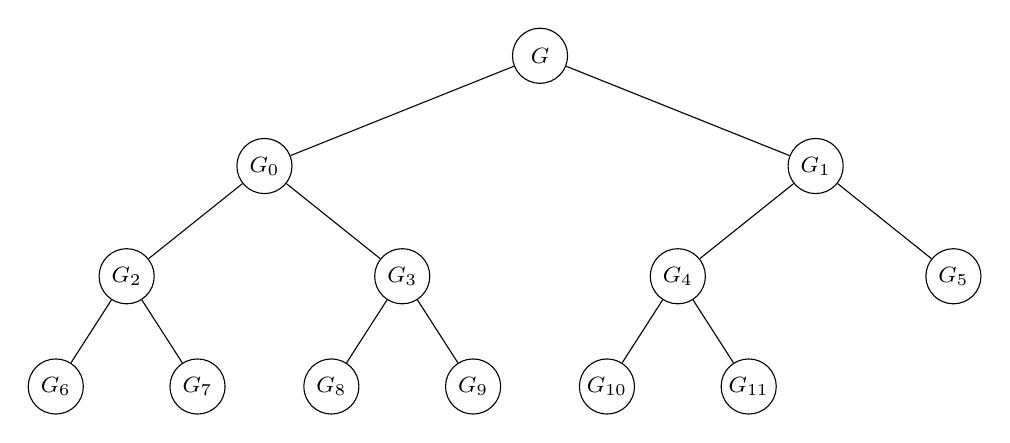
\begin{tikzpicture}[
	level distance=1.4cm,
	every node/.style={circle, draw, minimum size=7mm, inner sep=1pt, font=\footnotesize},
	edge from parent/.style={draw, -},
	level 1/.style={sibling distance=7cm},
	level 2/.style={sibling distance=3.5cm},
	level 3/.style={sibling distance=1.8cm},
	]
	
	\node {$G$}
	child {node {$G_0$}
		child {node {$G_{2}$}
			child {node {$G_6$}}
			child {node {$G_7$}}
		}
		child {node {$G_{3}$}
			child {node {$G_8$}}
			child {node {$G_9$}}
		}
	}
	child {node {$G_1$}
		child {node {$G_{4}$}
			child {node {$G_{10}$}}
			child {node {$G_{11}$}}
		}
		child {node {$G_{5}$}}
	};
	
\end{tikzpicture}
}
	\caption{The process of bisecting a graph into 7 partitions.}
	\label{fig:tree}
\end{figure}

During each bisecting step, GGP is used. As it was described in Section~\ref{graph_growing}, this bisection approach bases itself on BFS. Starting from a random seed it tries to group together vertices connected to each other. At every step it checks that both partitions maintain a weight threshold. Once a partition is computed the graph is further refined using the refinement algorithm proposed by Fiduccia and Mattheyses (FM) in \cite{fiduccia_fm}. The FM refinement algorithm goes through the boundary vertices of the graph, vertices that share at least one edge with a vertex in the other partition. For each step the vertex move that yields the greatest reduction in edge cut (see Section~\ref{subs:objective_functions}) is selected. In order to avoid a subpar solution, FM allows a limited number of moves that worsen the edge cut. This process is repeated over the boundary vertices several times, each time keeping the partition with the lowest edge cut.

It is worth noting that also for our volume based objective we have made use of this approach based on edge cut for the initial partition. There are a few reasons for this. Firstly, the initial partition is going to be heavily refined later during the uncoarsening phase, making the quality of the initial partition not as important. Additionally algorithms like FM are fast and work well with edge cut, optimizing for another objective would make this phase significantly slower. All of these reasons make it reasonable to use edge cut as an objective for this first partitioning.  

\section{Uncoarsening Phase}
The final step is the uncoarsening and refinement phase. During this phase our graph is gradually projected back to the original size. The vertices in a coarse vertex are automatically assigned to the same partition as the coarse vertex. 




%At each level the graph undergoes a refinement of the partitions to ensure better quality with the increased degree of freedom in the finer graph. 



 

%This section will present the multilevel approach as the most important in parallel computing\\
%Coarsening phase\\
%Initial partition \\
%Uncoarsening and refinement\\
%All the way with examples of how Metis is implemented, especially for the volume objective. 